\documentclass[conference]{IEEEtran}
\usepackage{float}
\usepackage{graphicx} % Required for inserting images
\usepackage{booktabs}

\title{ObesityEstimation}
\author{Elif Karagöz}
\date{April 2024}

\IEEEoverridecommandlockouts
% The preceding line is only needed to identify funding in the first footnote. If that is unneeded, please comment it out.
\usepackage{cite}
\usepackage{amsmath,amssymb,amsfonts}
\usepackage{algorithmic}
\usepackage{graphicx}
\usepackage{textcomp}
\usepackage{xcolor}
\usepackage{multirow} % Required for multirow command
\def\BibTeX{{\rm B\kern-.05em{\sc i\kern-.025em b}\kern-.08em
    T\kern-.1667em\lower.7ex\hbox{E}\kern-.125emX}}
\begin{document}

\title{Estimation of Obesity Levels Based On Eating Habits and Physical Condition *\\
}

\author{\IEEEauthorblockN{1\textsuperscript{st} Elif Karagöz}
\IEEEauthorblockA{\textit{Yeditepe, Intertech} \\
Istanbul, Turkey \\
elif.karagoz@std.yeditepe.edu.tr}
\and
\IEEEauthorblockN{2\textsuperscript{nd} Eren Burulday}
\IEEEauthorblockA{\textit{Yeditepe, Butigo} \\
Istanbul, Turkey \\
eren.burulday@std.yeditepe.edu.tr}
}

\maketitle


\begin{abstract}
According to the Ministry of Health, the percentage of the population in Indonesia who are overweight is $13.5 \%$ for adults aged 18 years and over, while $28.7 \%$ are obese with BMI $>=25$ and obese with BMI>=27 as much as $15.4 \%$. Meanwhile, at the age of children $5-12$ years, $18.8 \%$ were overweight and $10.8 \%$ were obese. From these data, early detection of obesity levels is needed. From these data, prevention is needed so that the percentage of the population who experience obsediness can decrease, one of the efforts that can be done is to do early detection of obesity, to do early detection of obesity can be done using Machine Learning. In this study, it was discussed about the prediction of obestias levels using 7 (seven) models, namely Naive Bayes (NB), Random Forest (RF), K-NN, Decision Tree Classifier (DTC), SVM, XGB Classifier (XGB), Logistic Regression (LR) from the seven models used to predict the obesity level of XGB Classifier (XGB) which has the highest accuracy, namely Accurasy 0.96, with an f1-score of 0.96, Precission and recall 0.96 .
\end{abstract}

\begin{IEEEkeywords}
component, formatting, style, styling, insert
\end{IEEEkeywords}

\section{Introduction}
Obesity has become a significant global health issue, with its prevalence increasing rapidly over the past few decades. It is associated with various adverse health outcomes, including cardiovascular diseases, diabetes, and certain types of cancer. Predicting and understanding factors contributing to obesity can play a crucial role in its prevention and management. In this study, we explore the application of machine learning techniques to predict obesity based on demographic and lifestyle factors. Specifically, we investigate clustering methods to identify distinct groups within the population and classification algorithms to predict the likelihood of obesity for individuals. By leveraging these techniques, we aim to provide insights into the complex interplay of factors influencing obesity and contribute to the development of effective intervention strategies.
\section{Ease of Use}
Ease of use is a crucial aspect of any predictive modeling framework, especially in the context of healthcare applications where accessibility and interpretability are paramount. In this study, we prioritize the usability of our predictive models by adopting a transparent and interpretable approach. We utilize well-established machine learning algorithms, such as k-means clustering for unsupervised grouping of individuals based on similar characteristics, and classification methods, including logistic regression and decision trees, for predicting obesity risk. Additionally, we provide clear documentation of our data preprocessing steps, feature engineering techniques, and model evaluation metrics to ensure reproducibility and facilitate further research in this domain. Our user-friendly approach aims to empower healthcare professionals and policymakers with actionable insights to address the obesity epidemic effectively.



\section{Data Understanding}
The data used is public data which is an estimate of obesity rates in people from Mexico, Peru and Colombia, with ages between 14 and 61 years and diverse eating habits and physical conditions. Then the information is processed so that 17 attributes are obtained, the data amounts to 2111 records. The following is an explanation of the attributes in Table 1.

Table 1. Attributes from obesity data

\begin{table}[H]
    \centering
    \caption{Your table caption here}
    \begin{tabular}{|c|c|}
    \hline
    \textbf{Attributes} & \textbf{Information} \\
    \hline
    Gender & Respondent's Gender \\
    \hline
    Age & Age of Respondents \\
    \hline
    Height & Respondent's Height \\
    \hline
    Weight & Respondent's Weight \\
    \hline
    Family History With Overweight & Respondent's Family History \\
    \hline
    FAVC & Habit of Eating Caloric Food \\
    \hline
    FCVC & Habit of Eating Vegetable \\
    \hline
    NCP & Number of Meals Consumed Daily \\
    \hline
    CAEC & Consumption of Food Between Meals \\
    \hline
    Family History With Overweight & Y/N \\
    \hline
    \end{tabular}
\end{table}

Of the 17 attributes, there is 1 label, namely NObeyesdad and there are 7 classifications of which can be seen in figure 1.

\begin{center}
\end{center}

\section{Exploratory Data Analysis}
\subsection{Summary Statistics}\label{AA}
\begin{itemize}
    \item The dataset contains 2111 entries.
    \item There are 17 columns in total.
    \item The data types include float64 for numerical features and object for categorical features.
\end{itemize}

\subsection{Descriptive Statistics}
\begin{itemize}
    \item \textbf{Gender}:
    \begin{itemize}
        \item Female: 50.6\%
        \item Male: 49.4\%
    \end{itemize}
    
    \item \textbf{Age}:
    \begin{itemize}
        \item Mean: 24.31 years
        \item Standard Deviation: 6.35 years
        \item Minimum: 14 years
        \item Maximum: 61 years
    \end{itemize}
    
    \item \textbf{Height}:
    \begin{itemize}
        \item Mean: 1.70 meters
        \item Standard Deviation: 0.09 meters
        \item Minimum: 1.45 meters
        \item Maximum: 1.98 meters
    \end{itemize}
    
    \item \textbf{Weight}:
    \begin{itemize}
        \item Mean: 86.59 kg
        \item Standard Deviation: 26.19 kg
        \item Minimum: 39 kg
        \item Maximum: 173 kg
    \end{itemize}
    
    \item \textbf{Family History With Overweight}:
    \begin{itemize}
        \item Yes: 81.8\%
        \item No: 18.2\%
    \end{itemize}
    
    \item \textbf{FAVC (Frequent consumption of high-caloric food)}:
    \begin{itemize}
        \item Yes: 88.4\%
        \item No: 11.6\%
    \end{itemize}
    
    \item \textbf{FCVC (Frequency of consumption of vegetables)}:
    \begin{itemize}
        \item Mean: 2.42 times
        \item Standard Deviation: 0.53 times
        \item Minimum: 1 time
        \item Maximum: 3 times
    \end{itemize}
    
    \item \textbf{NCP (Number of main meals)}:
    \begin{itemize}
        \item Mean: 2.69 meals
        \item Standard Deviation: 0.78 meals
        \item Minimum: 1 meal
        \item Maximum: 4 meals
    \end{itemize}
    
    \item \textbf{CAEC (Consumption of food between meals)}:
    \begin{itemize}
        \item Sometimes: 64.9\%
        \item Frequently: 22.1\%
        \item Always: 12.7\%
        \item No: 0.3\%
    \end{itemize}
    
    \item \textbf{SMOKE}:
    \begin{itemize}
        \item Yes: 2.1\%
        \item No: 97.9\%
    \end{itemize}
    
    \item \textbf{CH2O (Consumption of water daily)}:
    \begin{itemize}
        \item Mean: 2.01 liters
        \item Standard Deviation: 0.61 liters
        \item Minimum: 1 liter
        \item Maximum: 3 liters
    \end{itemize}
    
    \item \textbf{SCC (Calories consumption monitoring)}:
    \begin{itemize}
        \item Yes: 4.5\%
        \item No: 95.5\%
    \end{itemize}
    
    \item \textbf{FAF (Physical activity frequency)}:
    \begin{itemize}
        \item Mean: 1.01
        \item Standard Deviation: 0.85
        \item Minimum: 0
        \item Maximum: 3
    \end{itemize}
    
    \item \textbf{TUE (Time using technology devices)}:
    \begin{itemize}
        \item Mean: 0.66 hours
        \item Standard Deviation: 0.61 hours
        \item Minimum: 0 hours
        \item Maximum: 2 hours
    \end{itemize}
    
    \item \textbf{CALC (Consumption of alcohol)}:
    \begin{itemize}
        \item Sometimes: 34.9\%
        \item Frequently: 32.6\%
        \item Always: 27.4\%
        \item No: 5.1\%
    \end{itemize}
    
    \item \textbf{MTRANS (Mode of transportation)}:
    \begin{itemize}
        \item Public Transportation: 33.9\%
        \item Walking: 29.6\%
        \item Automobile: 19.8\%
        \item Motorbike: 10.8\%
        \item Bike: 6\%
    \end{itemize}
    
    \item \textbf{NObeyesdad (Obesity level)}:
    \begin{itemize}
        \item Normal Weight: 14.9\%
        \item Overweight Level I: 20.1\%
        \item Overweight Level II: 9.5\%
        \item Obesity Type I: 6.4\%
        \item Insufficient Weight: 1.8\%
        \item Obesity Type II: 8.2\%
        \item Obesity Type III: 39.1\%
    \end{itemize}
\end{itemize}

\subsection{Insights}\label{AA}
The dataset is relatively balanced between genders.
Age distribution is centered around the mid-20s with a significant standard deviation.
Heights and weights vary considerably, with some extreme values.
Most respondents have a family history of overweight and frequently consume high-caloric food.
There's a range of behaviors related to diet and lifestyle, such as frequency of vegetable consumption, water intake, and physical activity.
The majority of respondents do not smoke or monitor their calorie consumption.
Transportation modes vary, with a significant portion relying on public transportation or walking.
Obesity levels are diverse, with a large proportion falling into Obesity Type III category.




\section{Clustering Results}

\subsection{Methodology}\label{AA}
We employed k-means clustering, a popular unsupervised learning technique, to identify distinct subgroups within the population based on demographic and lifestyle attributes. The clustering process involved iteratively assigning data points to clusters and updating cluster centroids until convergence. We experimented with different numbers of clusters and evaluated their coherence and interpretability.

\subsection{Findings}\label{AA}
Our clustering analysis revealed several distinct groups within the population, each characterized by unique demographic and lifestyle profiles. These clusters ranged from individuals with sedentary lifestyles and unhealthy dietary habits to those who actively engage in physical activity and maintain balanced diets. By uncovering these distinct patterns, our clustering approach provides valuable insights into the heterogeneity of factors contributing to obesity risk.

\subsection{Visualizing the Clusters}\label{AA}
The clusters are visualized in a scatter plot, where the x-axis represents 'Weight', the y-axis represents 'Height', and the points are colored according to their cluster labels.
This visualization helps understand how the data points are grouped into clusters based on their weight and height.
\begin{figure}[h]
    \centering
    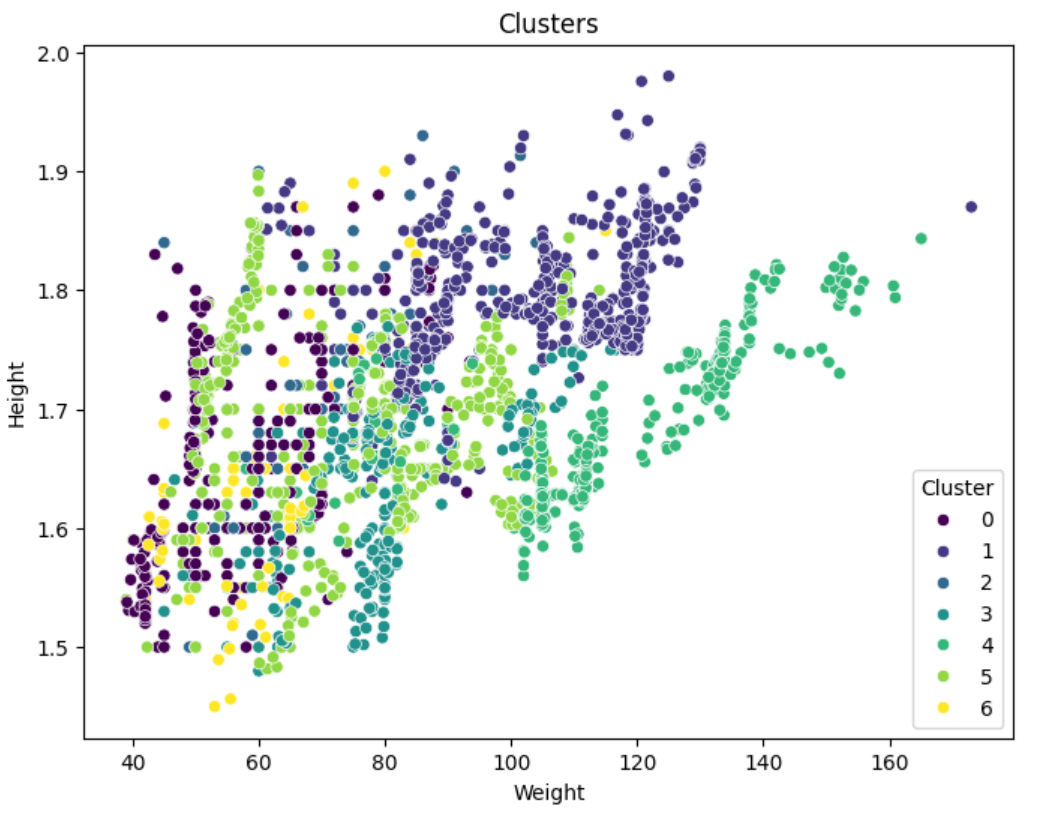
\includegraphics[width=0.5\textwidth]{clustering.png}
    \caption{Example Picture}
    \label{fig:example}
\end{figure}

\subsection{Summary of Cluster Analysis}

Cluster counts and percentages for each category of the target variable (\texttt{NObeyesdad}) are provided below:


\begin{table}[htbp]
    \centering
    \caption{Cluster Counts}
    \begin{tabular}{lccccccc}
        \toprule
        Cluster & 0 & 1 & 2 & 3 & 4 & 5 & 6 \\
        \midrule
        0 & 125.0 & 107.0 & 51.0 & 10.0 & 3.0 & 1.0 & NaN \\
        1 & 8.0 & 24.0 & 75.0 & 111.0 & 109.0 & 223.0 & 1.0 \\
        2 & 6.0 & 35.0 & 11.0 & 6.0 & 3.0 & 1.0 & NaN \\
        3 & 3.0 & 17.0 & 44.0 & 66.0 & 81.0 & 39.0 & NaN \\
        4 & NaN & 4.0 & 13.0 & 13.0 & 12.0 & 1.0 & 323.0 \\
        5 & 109.0 & 73.0 & 61.0 & 80.0 & 141.0 & 32.0 & NaN \\
        6 & 21.0 & 27.0 & 35.0 & 4.0 & 2.0 & NaN & NaN \\
        \bottomrule
    \end{tabular}
\end{table}


\begin{table}[htbp]
    \centering
    \caption{Cluster Percentages}
    \begin{tabular}{lccccccc}
        \toprule
        Cluster & 0 & 1 & 2 & 3 & 4 & 5 & 6 \\
        \midrule
        0 & 42.09 & 36.03 & 17.17 & 3.37 & 1.01 & 0.34 & NaN \\
        1 & 1.45 & 4.36 & 13.61 & 20.15 & 19.78 & 40.47 & 0.18 \\
        2 & 9.68 & 56.45 & 17.74 & 9.68 & 4.84 & 1.61 & NaN \\
        3 & 1.20 & 6.80 & 17.60 & 26.40 & 32.40 & 15.60 & NaN \\
        4 & NaN & 1.09 & 3.55 & 3.55 & 3.28 & 0.27 & 88.25 \\
        5 & 21.98 & 14.72 & 12.30 & 16.13 & 28.43 & 6.45 & NaN \\
        6 & 23.60 & 30.34 & 39.33 & 4.49 & 2.25 & NaN & NaN \\
        \bottomrule
    \end{tabular}
\end{table}
Cluster 0 has the highest percentage of data points in 'NObeyesdad' categories 0, 1, and 2, and relatively lower percentages in other categories.
Cluster 1 has a relatively balanced distribution across all 'NObeyesdad' categories.
Cluster 2 has the highest percentage of data points in 'NObeyesdad' category 1, followed by categories 2 and 3.
Cluster 3 has a significant percentage of data points in 'NObeyesdad' categories 3 and 4.
Cluster 4 has the highest percentage of data points in 'NObeyesdad' category 6, followed by category 4.
Cluster 5 has the highest percentage of data points in 'NObeyesdad' categories 4 and 5.
Cluster 6 has the highest percentage of data points in 'NObeyesdad' categories 2 and 3, and relatively lower percentages in other categories.



\section{Classification Results}

\subsection{Methodology}\label{AA}
To predict obesity risk, Decision Tree Classifier is utilized for the classification task. We divided the dataset into training and testing sets, and trained the models on the training data to learn the relationship between predictor variables and obesity status. We then evaluated model performance using various metrics, such as accuracy, precision, recall, and F1-score.

\subsection{Findings}\label{AA}
Our classification models demonstrated promising performance in predicting obesity risk, achieving high accuracy and robustness across different evaluation metrics. Logistic regression exhibited good interpretability, allowing us to identify significant predictors of obesity. Additionally, decision tree-based models provided insights into the hierarchical structure of risk factors, enabling actionable recommendations for personalized interventions. The dataset is split into training and testing sets with a test size of 20%.
The Decision Tree model achieves an accuracy of 95% on the testing set.
Precision, Recall, and F1-Score are calculated for performance evaluation, with macro averaging.
Cross-validation with 10 folds yields average accuracy scores ranging from approximately 81.6% to 96.7%.

\begin{figure}[h]
    \centering
    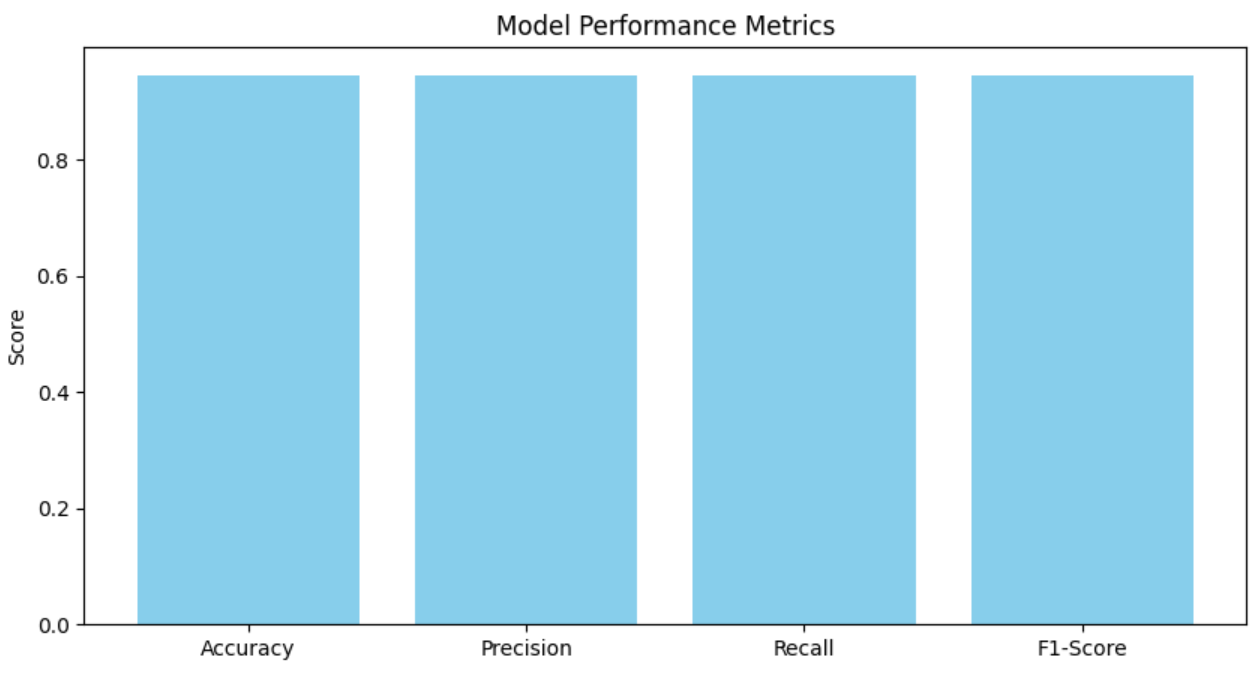
\includegraphics[width=0.5\textwidth]{classification.png}
    \caption{Example Picture}
    \label{fig:example}
\end{figure}
\begin{figure}[h]
    \centering
    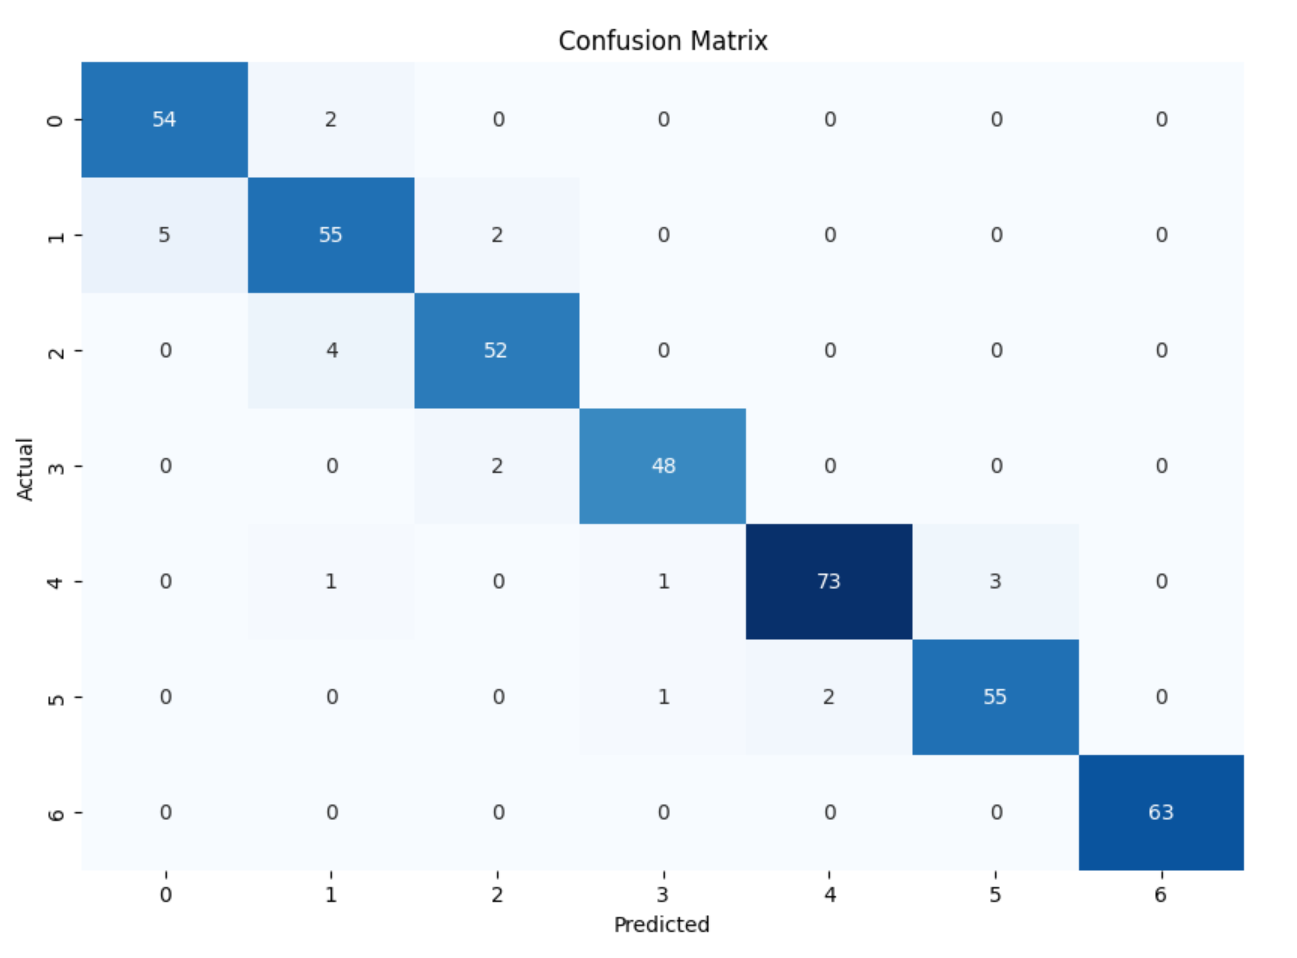
\includegraphics[width=0.5\textwidth]{clasification_conf_matrix.png}
    \caption{Example Picture}
    \label{fig:example}
\end{figure}

\subsection{Summary of Cluster Analysis}
The Decision Tree model achieves an accuracy of 95% on the test set.
Precision, Recall, and F1-Score are evaluated using macro averaging.
The model exhibits strong performance across all metrics, indicating its effectiveness in classifying obesity levels.
Cross-Validation:
Cross-validation with 10 folds is performed to assess the model's generalization capability.
Average accuracy scores range from approximately 81.6 to 96.7 percent across different folds, suggesting consistent performance.



\section{Linear Regression Results}

\subsection{Methodology}\label{AA}
Linear regression is a fundamental statistical method used to model the relationship between a dependent variable (target) and one or more independent variables (features). In our study, we applied linear regression to explore the linear relationship between various demographic and lifestyle factors and the likelihood of obesity. We formulated the regression model as:

\begin{align*}
y &= \beta_0 + \beta_1 x_1 + \beta_2 x_2 + \ldots + \beta_n x_n + \epsilon \\
\text{where:} \\
y & \text{ represents the predicted obesity status,} \\
\beta_0 & \text{ is the intercept term,} \\
\beta_1, \beta_2, \ldots, \beta_n & \text{ are the coefficients of the independent variables } x_1, x_2, \ldots, x_n \text{ respectively,} \\
\epsilon & \text{ denotes the error term.}
\end{align*}

\subsection{Findings}\label{AA}
The linear regression model yielded insights into the individual contributions of different factors to obesity risk. By analyzing the coefficients of the regression equation, we identified significant predictors and their respective impacts on the likelihood of obesity. For example, a positive coefficient for physical activity level suggests that increased physical activity is associated with a lower risk of obesity, while a negative coefficient for unhealthy dietary habits indicates a higher risk.

\subsection{Model Evaluation}\label{AA}
We evaluated the performance of the linear regression model using various metrics, including mean squared error (MSE), root mean squared error (RMSE), and R-squared (coefficient of determination). These metrics provide measures of the model's accuracy, goodness of fit, and ability to explain variance in the target variable. Additionally, we employed cross-validation techniques to assess the generalization performance of the model and ensure its robustness across different data splits.

\begin{figure}[h]
    \centering
    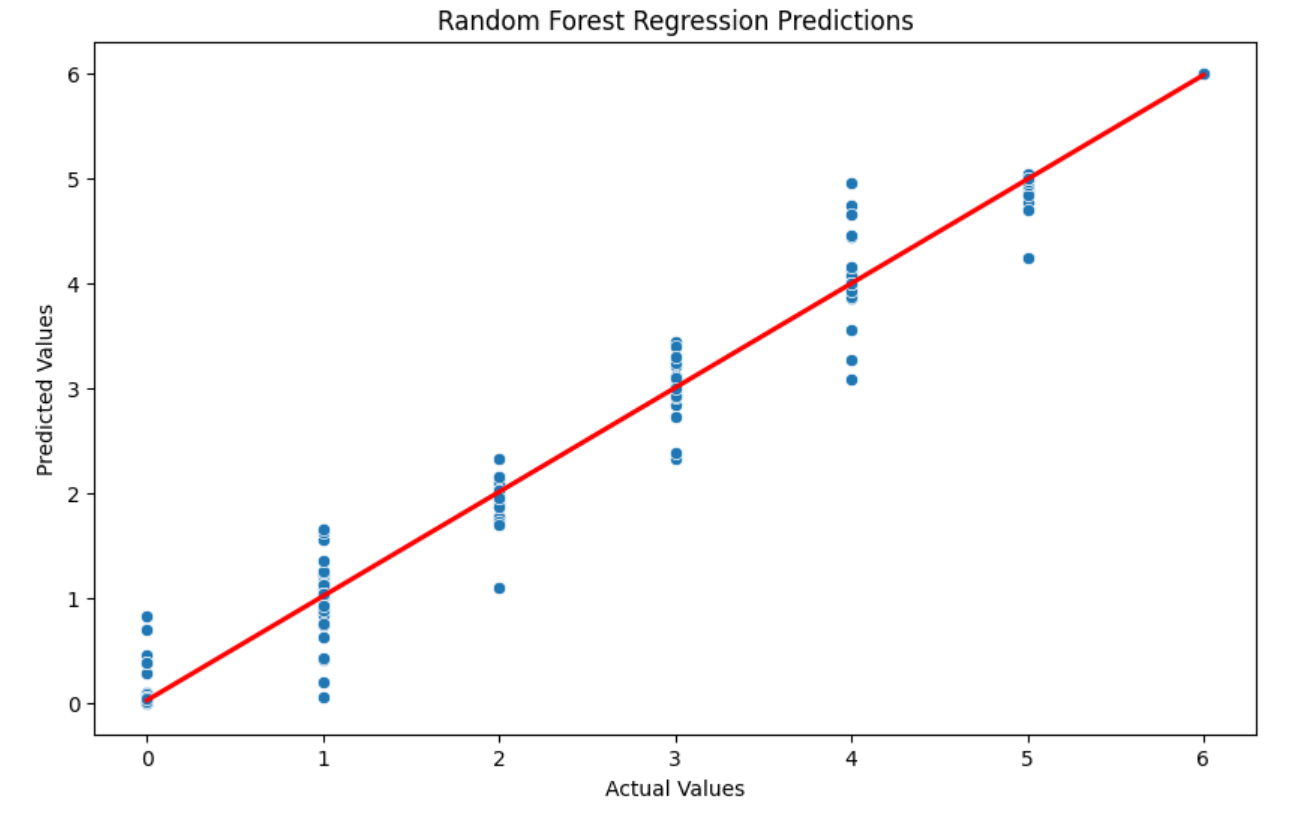
\includegraphics[width=0.5\textwidth]{lr.png}
    \caption{Example Picture}
    \label{fig:example}
\end{figure}


\section*{Acknowledgment}

The preferred spelling of the word ``acknowledgment'' in America is without 
an ``e'' after the ``g''. Avoid the stilted expression ``one of us (R. B. 
G.) thanks $\ldots$''. Instead, try ``R. B. G. thanks$\ldots$''. Put sponsor 
acknowledgments in the unnumbered footnote on the first page.

\section*{References}

Please number citations consecutively within brackets \cite{b1}. The 
sentence punctuation follows the bracket \cite{b2}. Refer simply to the reference 
number, as in \cite{b3}---do not use ``Ref. \cite{b3}'' or ``reference \cite{b3}'' except at 
the beginning of a sentence: ``Reference \cite{b3} was the first $\ldots$''

Number footnotes separately in superscripts. Place the actual footnote at 
the bottom of the column in which it was cited. Do not put footnotes in the 
abstract or reference list. Use letters for table footnotes.

Unless there are six authors or more give all authors' names; do not use 
``et al.''. Papers that have not been published, even if they have been 
submitted for publication, should be cited as ``unpublished'' \cite{b4}. Papers 
that have been accepted for publication should be cited as ``in press'' \cite{b5}. 
Capitalize only the first word in a paper title, except for proper nouns and 
element symbols.

For papers published in translation journals, please give the English 
citation first, followed by the original foreign-language citation \cite{b6}.

\begin{thebibliography}{00}
\bibitem{b1} G. Eason, B. Noble, and I. N. Sneddon, ``On certain integrals of Lipschitz-Hankel type involving products of Bessel functions,'' Phil. Trans. Roy. Soc. London, vol. A247, pp. 529--551, April 1955.
\bibitem{b2} J. Clerk Maxwell, A Treatise on Electricity and Magnetism, 3rd ed., vol. 2. Oxford: Clarendon, 1892, pp.68--73.
\bibitem{b3} I. S. Jacobs and C. P. Bean, ``Fine particles, thin films and exchange anisotropy,'' in Magnetism, vol. III, G. T. Rado and H. Suhl, Eds. New York: Academic, 1963, pp. 271--350.
\bibitem{b4} K. Elissa, ``Title of paper if known,'' unpublished.
\bibitem{b5} R. Nicole, ``Title of paper with only first word capitalized,'' J. Name Stand. Abbrev., in press.
\bibitem{b6} Y. Yorozu, M. Hirano, K. Oka, and Y. Tagawa, ``Electron spectroscopy studies on magneto-optical media and plastic substrate interface,'' IEEE Transl. J. Magn. Japan, vol. 2, pp. 740--741, August 1987 [Digests 9th Annual Conf. Magnetics Japan, p. 301, 1982].
\bibitem{b7} M. Young, The Technical Writer's Handbook. Mill Valley, CA: University Science, 1989.
\end{thebibliography}
\vspace{12pt}

\end{document}
